%!TEX TS-program = pdflatex
\documentclass[a4paper,12pt]{article}

\usepackage{mathptmx}
\usepackage{parskip}
\usepackage[top=1.5in,left=1in,right=1in,bottom=1in]{geometry}
%\setlength{\parindent}{0pt}
%\setlength{\parskip}{\the\baselineskip}
\pagestyle{empty} 

\makeatletter
\renewcommand\@makefntext[1]{%
  \parindent 1em\noindent
  \hbox{\@makefnmark}#1}
\renewcommand\large{\@setfontsize\large{14pt}{18}} % For standardizing with the Word template: normally \large is 14.4pt
\makeatother
\usepackage{titlesec}
\titleformat{\subsection}{\normalfont\normalsize}{\thesubsection.}{1ex}{}
\titleformat{\subsubsection}{\normalfont\normalsize}{\thesubsubsection.}{1ex}{}
\titleformat{\section}{\normalfont\normalsize\bfseries}{\thesection.}{1ex}{}
\titlespacing*{\section}{0pt}{*0}{0pt}
\titlespacing*{\subsection}{0pt}{\the\baselineskip}{0pt}

\usepackage{natbib} 
\bibpunct{(}{)}{;}{a}{,}{,}

\def\bad{{\leavevmode\llap{*}}}
\def\marginal{{\leavevmode\llap{?}}}
\def\verymarginal{{\leavevmode\llap{??}}}
\def\swmarginal{{\leavevmode\llap{4}}}
\def\infelic{{\leavevmode\llap{\#}}}

\newcommand{\6}{\mbox{$[\hspace*{-.6mm}[$}} 
\newcommand{\9}{\mbox{$]\hspace*{-.6mm}]$}}
\newcommand{\sem}[2]{\6#1\9$^{#2}$}
\newcommand{\mes}[1]{\6#1\9}

\RequirePackage[hyphens]{url}
\usepackage{enumitem,xcolor,color,graphbox,amsmath,amssymb,float,subcaption,hyperref,gb4e}
%\PassOptionsToPackage{hyphens}{url}\usepackage{hyperref}
%\usepackage[hyphens]{url}

\newcommand{\citepos}[1]{\citeauthor{#1}'s \citeyear{#1}}
\newcommand{\citetpos}[1]{\citeauthor{#1}'s (\citeyear{#1})}

\setlength{\bibsep}{0pt} \relax
\setcitestyle{notesep={: },yysep={, }} \relax

\begin{document}

{\large \textbf{On the information structure sensitivity of projective content}}\footnote{We thank Taylor Mahler, Julie McGory and Elena Vaik\v{s}norait\.{e} for assistance in creating the stimuli, as well as the participants of {\em Sinn und Bedeutung} 2018 for critical feedback on the material presented here. We also gratefully acknowledge financial support from National Science Foundation grant BCS-1452674 (JT) and The Ohio State University Targeted Investment in Excellence (MCdM, JT). Jon Stevens was supported by a postdoctoral fellowship awarded to Marie-Catherine de Marneffe and Judith Tonhauser from the American Council of Learned Societies and the OSU Arts \& Sciences Discovery Theme during the year that we designed and ran the experiment.}\\
Judith TONHAUSER --- \textit{The Ohio State University, Stuttgart University}\\
Marie-Catherine DE MARNEFFE --- \textit{The Ohio State University}\\
Shari R.\ SPEER --- \textit{The Ohio State University}\\
Jon STEVENS --- \textit{The Ohio State University}\\

\textbf{Abstract.} This paper presents the findings of an experiment designed to investigate the information structure sensitivity of the projective contents associated with {\em again, stop} and manner adverbs. In contrast to the prejacent of manner adverbs, whose projectivity is expected to be sensitive to information structural focus (e.g., \citealt{abrusan2013,stevens-etal2017}), that of the prejacent of {\em again} is not (e.g., \citealt{beck2006,abrusan2013b}). We also investigated the pre-state content associated with {\em stop} because projection analyses differ in their predictions regarding the sensitivity of this projective content to information structural focus (e.g., \citealt{heim83,vds92,kadmon01,simons01,abrusan2011,abrusan2016,romoli2011,romoli2015}). We found that the projectivity of all three contents is sensitive to prosodically marked focus and discuss the implications of our findings for empirically adequate projection analyses.

\textbf{Keywords:} projective content, presuppositions, {\em stop, again}, manner adverbs, focus, prosody

% deadline Jan 31: send manuscript to sinnub23@gmail.com with "SuB23 Proceedings: FIRST-AUTHOR-LASTNAME" as the subject 
% send TEX, PDF, BIB and all figures
% no strict length restriction, but around 24 pages including everything

\section{Introduction}\label{s1}

Projective content is utterance content that is said to `project' over entailment-canceling operators; that is, projective content is utterance content that listeners may take speakers to be committed to even when the expression associated with the content occurs in an entailment-canceling environment (e.g., \citealt*{ccmg90,potts05,brst-ar}). To illustrate, consider the examples in (\ref{again}) and (\ref{manner}). A speaker who utters the sentence in (\ref{again}a) is typically taken to be committed to the content that Sam visited Barcelona at least once before July 2018. Because a speaker who utters the polar question variant in (\ref{again}b) may also be taken to be committed to this content, this content is considered projective content. Similarly, a speaker who utters the manner adverb sentence in (\ref{manner}a) with prosodic prominence on the manner adverb {\em wildly} (indicated by capital letters) is typically taken to be committed to the content that Sam shouted. Because a speaker who utters the variant in (\ref{manner}b) may also be taken to be committed to this content, it is considered projective.

\begin{exe}
\ex\label{again}
\begin{xlist}
\ex In early July 2018, Sam visited Barcelona again.

\ex Did Sam visit Barcelona again in early July 2018? 
\end{xlist}

\ex\label{manner}

\begin{xlist}
\ex At the dinner party, Sam shouted WILDLY.

\ex Did Sam shout WILDLY at the dinner party?
\end{xlist}
\end{exe}

Why is some utterance content projective and how can projectivity be formally derived? Over the past decades, several different answers have been given to these questions (for overviews see, e.g., \citealt{kadmon01,brst-salt10,beaver-geurts-sep}, and references therein). On one of the most widely adopted analyses, content is projective because it is lexically specified as presupposed: this means that the content must be entailed by or satisfied in the common ground of the interlocutors prior to interpretation of the sentence that realizes the triggering expression (e.g., \citealt{heim83,vds92}). Such a lexicalist analysis is often adopted for the projective content associated with {\em again} (or German {\em wieder} `again'; e.g., \citealt{kamp-rossdeutscher1994,fabricius-hansen2001,simons01,jaeger-blutner2003,vds-huitink2003,beck2006}; but see \citealt{abrusan2013b,abrusan2016}); we henceforth refer to the projective content associated with {\em again} as the prejacent. Consider, for instance, the lexical entry for {\em again} proposed by \citet{beck2006}, where $t'$ is an anaphorically retrieved time,\footnote{Even though the prejacent of {\em again} features a temporal anaphor, it is nevertheless assumed that the prejacent of {\em again} can be accommodated. For instance, \citet[fn.5]{beck2006} assumed that the prejacent of {\em again} is accommodated in her example (47a) {\em In the fall of 1997, they were in Riva. The next fall, they were on the AXALP again}. Naturally occurring examples also show that the prejacent of {\em again} can be accommodated. Headlines, for instance, can feature {\em again} without wreaking interpretative havoc: from the headline in (i) we can infer without trouble that The Cure has headlined Glastonbury before. For experimental investigations of the accommodation of the prejacent see \citealt{tiemann-thesis,tiemann-etal2015} and \citealt{bacovcin-etal2018}.

\begin{exe}
\exi{(i)} Could The Cure headline Glastonbury again? 
\\ \url{www.radiox.co.uk/artists/cure/robert-smith-talks-cure-headline-glastonbury/}
\end{exe}
} 
$p$ is the content of the sentence radical (that Sam visited Barcelona in (\ref{again})), and $t$ and $w$ are the time and world of evaluation, respectively:\footnote{In addition to the repetitive interpretation, {\em again} can give rise to a restitutive interpretation. Section \ref{s4} briefly considers the observed interaction between focus and the two interpretations of {\em again} (see, e.g., \citealt{beck2006}).}

\begin{exe}
\ex\label{beck} \mes{{\em again}}$(t')(p)(t)(w)$ is defined if and only if $p(t')(w)$ \& $t' < t$. \\ If defined, \mes{{\em again}}$(t')(p)(t)(w)$ = 1 if and only if $p(t)(w)$. \\ \hspace*{.2cm} \hfill (adapted from \citealt[286]{beck2006})
\end{exe}
According to this lexical entry, the meaning of (\ref{again}a) is defined if and only if $p$, that Sam visited Barcelona, holds at the contextually given time $t'$ and the world of evaluation $w$, and the contextually given time $t'$ temporally precedes $t$, here early July 2018. In other words, in (\ref{again}a), {\em again} triggers the presupposition that Sam visited Barcelona before early July 2018. If the presupposed prejacent is satisfied in or entailed by the relevant context, (\ref{again}a) is true if and only if Sam visited Barcelona in early July 2018. Because {\em again} introduces the same presupposition in the polar question in (\ref{again}b), a speaker who utters the polar question is likewise predicted to be taken to be committed to Sam having visited Barcelona before early July 2018. %(Other analyses of the presupposed prejacent of {\em again} are considered in the context of our experiment findings in section \ref{s4}.)

A lexicalist analysis is generally not adopted for the projective content of manner adverbs, which is also referred to as the prejacent; in (\ref{manner}), for instance, the prejacent is that Sam shouted. Instead, the projectivity of the prejacent is derived from focus (e.g., \citealt{abrusan2013}, \citealt*{stevens-etal2017}). For instance, \citet{stevens-etal2017} followed \citealt{best-question} in assuming, first, that utterance content projects if it is entailed by the Question Under Discussion (QUD) addressed by the utterance and, second, that information structural focus constrains the QUD addressed by the utterance. Thus, in a polar question like (\ref{manner}b) {\em Did Sam shout WILDLY at the dinner party?}, prosodic prominence on the manner adverb {\em wildly} provides a cue to the manner adverb being in focus, which in turn constrains the (possibly implicit) QUD to something like `How did Sam shout at the dinner party?'. This QUD is assumed to denote the set of  propositions \{Sam shouted x at the dinner party $|$ x is a property of events\}.  \citet{stevens-etal2017} also followed \citealt{best-question} in assuming that a set of propositions $P$ entails a proposition $p$ if and only if every proposition in $P$ entails $p$. Thus, because \{Sam shouted x at the dinner party $|$ x is a property of events\} entails the proposition that Sam shouted at the dinner party, a speaker who utters the polar question in (\ref{manner}b) can be taken to be committed to this content, i.e., the prejacent is projective. 

As illustrated above, different projection analyses are assumed for the prejacent of {\em again} and the prejacent of manner adverbs: a lexicalist one for the former and a focus-based one for the latter. This analytic difference is motivated by (at least) two properties on which the two prejacents differ: i) the extent to which they are projective (see \citealt*{tbd-variability} for evidence that projectivity is a gradient property of utterance content) and ii) whether their projectivity is sensitive to information structural focus. Regarding the first property, the prejacent of {\em again} is assumed to be highly projective, whereas the projectivity of the prejacent of manner adverbs is assumed to be weaker. For instance, the prejacent of {\em again} is typically assumed to be non-suspendable in explicit ignorance contexts (e.g., \citealt{simons01,abrusan2016}), as shown by the unacceptability of  (\ref{suspend}a); as a consequence, {\em again} is typically considered a `hard trigger' (e.g., \citealt{simons01,abusch10,abrusan2016}). In contrast, the prejacent of manner adverbs can be suspended in such contexts, as shown by the acceptability of (\ref{suspend}b). 

\begin{exe}
\ex\label{suspend} 
\begin{xlist}
\ex {[}The speaker observes Jane, whose history of video rental she knows nothing about, in a video store.] \\ \infelic I have no idea whether Jane ever rented ``Manhattan'', but perhaps she is renting it again. \hfill (\citealt[433]{simons01})

\ex I have no idea whether Sam shouted at the dinner party, but if he shouted WILDLY, he will never be invited again.

\end{xlist}

%\ex footnote 3 in Abrusan 2016 reports intuitions by reviewer that examples with again are better than with too

\end{exe}
This difference in projectivity is taken to be captured by giving different analyses of the prejacent of {\em again} and of manner adverbs. By analyzing the prejacent of {\em again} as a lexically triggered presupposition with an anaphoric component (the time $t'$ in (\ref{beck})), the prejacent of {\em again} is predicted to be highly projective and not suspendable. By contrast, projective content that is derived from prosodically marked information structural focus, like the prejacent of manner adverbs, is predicted to be more weakly projective, for several reasons: first, prosodic cues to focus are non-deterministic, thereby potentially resulting in uncertainty on part of the listener on which expression is focused and, hence, which QUD the utterance addresses; second, focus constrains the QUD but doesn't determine it, thereby again potentially resulting in uncertainty on part of the listener about the QUD; third, focus-induced projectivity can be overridden by  contextual information about the speaker's epistemic state (see also \citealt{abrusan2011}).

A second property on which the prejacents of {\em again} and manner adverbs are taken to differ is in the sensitivity of their projectivity to information structural focus: the projectivity of the prejacent of manner adverbs is assumed to be sensitive to information structural focus, in contrast to that of the prejacent of {\em again} (e.g., \citealt{beck2006,abrusan2013,abrusan2013b}). A focus-based projection analysis for the prejacent of manner adverbs straightforwardly predicts that the projectivity of the prejacent is sensitive to what is focused in the utterance. For instance, if the subject of the polar question in (\ref{manner}b) is focused, as in {\em Did SAM shout wildly at the dinner party?}, then the QUD of the discourse may be the set of propositions \{x shouted wildly at the dinner party $|$ x a person\}. Because this QUD does not entail that Sam shouted (e.g., the proposition that Sue shouted wildly at the dinner party does not entail that Sam shouted), the prejacent of the manner adverb is not predicted to project. In contrast, the projectivity of a lexically specified presupposition is not expected to be sensitive to information structural focus (for discussion, see \citealt{djaerv-bacovcin-salt27} and section \ref{s4}).

In sum, these differences between the prejacents of {\em again} and manner adverbs provide empirical motivation for distinct projection analyses. These properties may  also help decide between competing analyses of other projective contents. A case in point is the pre-state content of {\em stop}, for which several different projection analysis have been proposed. This projective content is illustrated in the examples in (\ref{stopN}). A speaker who utters the sentence in (\ref{stopN}a) is typically taken to be committed to Sam having photographed the Sagrada Familia. Because a speaker who utters the polar question in (\ref{stopN}b) may likewise be taken to be committed to Sam having photographed the Sagrada Familia, this content, referred to as the pre-state content, is projective.

\begin{exe}
\ex\label{stopN}
\begin{xlist}
\ex Sam stopped photographing the Sagrada Familia.

\ex Did Sam stop photographing the Sagrada Familia?
\end{xlist}
\end{exe}
The pre-state content of {\em stop} has traditionally been analyzed as a lexically specified presupposition (e.g., \citealt{heim83,vds92,kadmon01}). More recently, alternative analyses have been proposed. On Abusch's (2002, 2010)  and Romoli's (2011, 2015) analyses, for instance, the projectivity of the pre-state content of {\em stop} is derived from conventionally specified alternatives to {\em stop} (these analyses differ in their details, as discussed in section \ref{s4}.)  \citet{abrusan2011,abrusan2016}, in turn, proposed that the pre-state content projects because it is by default backgrounded, and \citet*{brst-ar} suggested that the pre-state content projects if and only if it is not at-issue with respect to the QUD (see also \citealt*{brst-salt10,tbd-variability}). 

These analyses differ in their predictions regarding the projectivity of the pre-state content of {\em stop} and its sensitivity to information structural focus. Regarding projectivity, for instance, the pre-state content is predicted to be more projective if it is lexically specified as a presupposition than if its projectivity is mitigated by the extent to which it is not at-issue, as on \citetpos{abrusan2016} or \citetpos{brst-ar} analyses. Similarly for information structure sensitivity: on a lexicalist analysis, we may expect the pre-state content to be less sensitive to information structural focus compared to an analysis on which projectivity is derived from information structural properties of the utterance, as in \citealt{abrusan2016} or \citealt{brst-ar}. 

The experiment reported on in this paper was designed to investigate the projectivity of the prejacent of {\em again}, the prejacent of manner adverbs and the pre-state content of {\em stop}, as well as the information structure sensitivity of their projectivity, with the goal of identifying which projection analyses are empirically adequate for these contents. There is already some preliminary experimental evidence in support of a lexicalist analysis of the prejacent of {\em again} and a focus-based analysis of the prejacent of manner adverbs. First, there is experimental support for the prediction of lexicalist analyses that the prejacent of German {\em wieder} `again' is highly projective (we are not aware of an experiment that investigated the projectivity of {\em again}).\footnote{The prejacent of  {\em wieder} `again' and {\em again} have been experimentally investigated: see, e.g., \citealt{schwarz-tiemann2012} and \citealt{jouravlev-etal2016} on its processing,  \citealt{tiemann-thesis,tiemann-etal2015} and \citet{bacovcin-etal2018} on whether it is accommodated, and \citealt{zehr-schwarz2018} on whether it is entailed.} Specifically, \citet{xue-onea11} found that the prejacent of {\em wieder} `again' is highly projective compared to the prejacent of {\em auch} `too' and the contents of the complements of {\em erfahren} `find out' and {\em wissen} `know'. Their participants read sentences like (\ref{thomas}) in which the presupposition trigger occurred in the antecedent of a conditional and were asked whether it is possible that the presupposition is false: e.g., whether it is possible that Thomas hasn't made sushi before.

\begin{exe}
\ex\label{thomas} \gll Wenn Thomas wieder Sushi macht, hilft Maiko dabei. \\ if Thomas again sushi makes helps Maiko with.it \\ \glt `If Thomas  makes sushi again, Maiko will help him.' \\ \hspace*{.2cm} \hfill (\citealt[176]{xue-onea11}; glosses added)
\end{exe}
Participants responded `no' in 101 (99\%) of the 102 trials with {\em wieder} `again', suggesting that the prejacent of {\em wieder} `again' is highly projective compared to the relevant contents of {\em auch} `too' (87\% `no'), {\em erfahren} `find out' (52\% `no') and {\em wissen} `know' (38\% `no'). This finding supports a lexicalist analysis of the prejacent of {\em wieder} `again'.

Second, there is experimental support for the prediction of focus-based analyses that the prejacent of manner adverbs is weakly projective and that its projectivity is sensitive to information structural focus. \citet*{stevens-etal2017} investigated the projectivity of the prejacent of English manner adverbs, as in (\ref{amanda}), in two prosodic conditions: with a L+H* pitch accent on the proper name or on the manner adverb. They assumed that the foci of the utterances were constrained by the position of the pitch accent. Participants assessed whether the speaker is certain of the prejacent; in (\ref{amanda}), that Amanda clapped.

\begin{exe}
\ex\label{amanda} Amanda didn't clap loudly.
\end{exe}
The mean ratings were 4.8 (out of 7) with a L+H* pitch accent on the proper name and 5.7 with a L+H* pitch accent on the manner adverb. Thus, \citet{stevens-etal2017} found that the prejacent of manner adverbs was only weakly projective and that its projectivity was sensitive to the prosodic manipulation of information structural focus. 

There also is empirical evidence that the pre-state content of {\em stop} is not highly projective. \citet{tbd-variability} investigated the projectivity of  projective contents associated with 19 English expressions, including the pre-state content of {\em stop}. Their Experiment 1a found that the projectivity of the pre-state content of {\em stop} is not at ceiling, in contrast to, for instance, the content of non-restrictive relative clauses, and significantly less projective than, for instance, the content of the complement of {\em know}. This finding is more compatible with analyses that assume that {\em stop} is a `soft trigger' (e.g., \citealt{simons01,abusch02,abusch10,romoli2011,romoli2015}) than with ones that assume that it is a `hard trigger' (e.g., \citealt{kadmon01}) or ones that take the pre-state content to be less susceptible to suspension than `soft triggers' (\citealt{abrusan2016}).

Despite these experimental findings, the currently available empirical evidence is insufficient to evaluate the empirical adequacy of the various analyses of the projective contents of {\em again}, manner adverbs and {\em stop}. For one, there has not been an experimental investigation of the projectivity of the prejacent of {\em again}.\footnote{The experiment reported on in \citealt{cummins-rohde2015} investigated both the pre-state content of {\em stop} and the prejacent of {\em again} with respect to whether prosodically signalled differences in the QUD influence presupposition projection. This work did not compare the 20 presuppositions investigated, but Figure 2 in this work suggests that the pre-state content of {\em stop} is at least numerically) more projective in the focus condition than in the neutral condition, whereas the opposite is true for the prejacent of {\em again}.} Furthermore, comparing the findings of the projection experiments reported on in \citealt{xue-onea11,stevens-etal2017} and \citealt{tbd-variability} is hampered by the fact that they used different response tasks to assess projectivity. Finally, information structure sensitivity has, to date, only been investigated for the prejacent of manner adverbs (\citealt{stevens-etal2017}), but not for the prejacent of {\em again} or the pre-state content of {\em stop}. The experiment reported on in this paper aims to contribute to filling these empirical gaps.

\section{Methods}\label{s2}

The experiment we report on was designed to address the research questions in (\ref{rqs}):

\begin{exe}
\ex\label{rqs} Regarding the prejacent of {\em again}, the prejacent of manner adverbs and the pre-state content of {\em stop}:
\begin{xlist}

\ex How projective are these contents?

\ex Is the projectivity of these contents sensitive to information structural focus?

\end{xlist}

\end{exe}

Projectivity was assessed using the `certain that' diagnostic for projection (see also, e.g., \citealt{tonhauser-salt26,djaerv-bacovcin-salt27,tbd-variability,mahler-nels}): under this diagnostic, participants are presented with utterances, like (\ref{sample}), and asked whether the speaker is certain of some content. For instance, to investigate the prejacent of the manner adverb in (\ref{sample}), participants are asked whether Debby is certain that Alfie texted. 

\begin{exe}
\ex\label{sample} Debby: Did Alfie text secretly?
\end{exe}

To compare the projectivity of the three contents, we have to consider their temporal properties: the prejacent of {\em again} and the pre-state content of {\em stop} invoke a time that temporally precedes the main clause event time, in contrast to the prejacent of manner adverbs. For instance, the prejacent of {\em again} in (\ref{sample22}a) and the pre-state content of {\em stop} in (\ref{sample22}b) is that Alfie texted before noon. By contrast, the prejacent of the manner adverb in (\ref{sample22}c) is that Alfie texted at noon.

\begin{exe}

\ex\label{sample22}

\begin{xlist}

\ex Did Alfie text again at noon?

\ex Did Alfie stop texting at noon?

\ex Did Alfie text secretly at noon?

\end{xlist}

\end{exe}
To facilitate comparison of the projective contents associated with the three expressions under investigation, the stimuli in our experiment were utterances of polar questions like (\ref{sample2}) in which temporal adjunct clauses constrained the relevant times. Crucially, the stimuli realized {\em when-}clauses with {\em again} and {\em stop}, and {\em before-}clauses with manner adverbs. As a consequence, our experiment investigated the same projective content for the three expressions; in (\ref{sample2}), for instance, the projective content for all three expressions is that Alfie texted before Dan arrived.

\begin{exe}

\ex\label{sample2}

\begin{xlist}

\ex Did Alfie text again when Dan arrived? 

\ex Did Alfie stop texting when Dan arrived? 

\ex Did Alfie text secretly before Dan arrived? 

\end{xlist}

\end{exe}
The experiment collected gradient certainty ratings for the projective contents associated with {\em again}, manner adverbs and {\em stop}. The full set of materials, the code for the analyses and figures, and a link to the experiment are provided in a GitHub repository at \url{https://github.com/judith-tonhauser/projectivity-and-focus-sensitivity}.

\subsection{Participants}

176 participants with U.S.\ IP addresses and at least 99\% of previous HITs approved were recruited on Amazon's Mechanical Turk platform (ages: 20-76; mean age: 36; 85 women, 91 men). They were paid \$1.20 for participating in the experiment. 

\subsection{Materials}

The target stimuli were 432 utterances of 108 polar questions consisting of a main clause and an adjunct clause, like those in (\ref{sample2}). As discussed above, the adjunct clauses for polar questions with {\em again} and {\em stop} were introduced by {\em when}, and the adjunct clauses for polar questions with manner adverbs were introduced by {\em before}. The polar questions featured 12 verbs, namely {\em text}, shown in (\ref{sample2}), as well as {\em clean, shout, yell, bark, knock, whistle, speak, walk, smile, cry} and {\em giggle}. We combined each of these verbs with 3 proper name subjects and adjunct clauses, for a total of 36 triples of polar questions like (\ref{sample2}), i.e., a total of 108 polar questions. The full set of polar questions is provided in Appendix A of the GitHub repository.

The adjunct clauses that each main clause verb was combined with were minimal variants of one another, e.g., the variants of {\em Dan arrived} in (\ref{sample2}) in the other 2 triples with {\em text} were {\em Kim showed up} and {\em Tom walked in}. In the manner adverb polar questions, the verb of the main clause was combined with a unique manner adverb: {\em text}, for instance, only occurred with {\em secretly}. The manner adverbs were chosen so that it is possible for the event described by the verb to be carried out in the manner described by the adverb, as well as not in that manner: for instance, it is possible to text secretly, and it is possible to text not secretly. This was done because \citet{stevens-etal2017} found that the projectivity of the prejacent of negated sentences with {\em smile cheerfully} (e.g., that Sandy smiled, in {\em Sandy didn't smile cheerfully}) was comparatively lower; we hypothesized that this was due to it being difficult for somebody who doesn't smile cheerfully to smile at all.

The position of information structural focus was manipulated prosodically: we recorded each of the 108 polar questions in four conditions, as illustrated in (\ref{sampleP}): a low pitch accent (L* in ToBI, the Tones and Break Indices annotation system, \citealt{beckman-ayers97}) was realized on the auxiliary, as in (\ref{sampleP}a), the proper name subject, as in (\ref{sampleP}b),  the verb, as in (\ref{sampleP}c), or the target expression, {\em again}, as in (\ref{sampleP}d); in target stimuli with {\em stop} or a manner adverb, the low pitch accent was realized on {\em stop} or the manner adverb in the target condition. The L* pitch accent was the only one realized in the utterance.\footnote{We used a L* rather than a H* pitch accent to mark focus because the former has been described as less biasing in polar questions than the latter (e.g., \citealt[290ff.]{pierrehumbert-hirschberg1990}).} The pitch contour after the L* pitch accent was high and relatively flat, and ended with an increase in f0, i.e., a H-H\% boundary tone.
 
\begin{exe}
\ex\label{sampleP} Four focus conditions, illustrated for the polar question in (\ref{sample2}a)\footnote{While we describe the tune realized on our target stimuli as L* H-H\% here, it is also possible to describe it as L*+H H-H\%, i.e., with a L*+H pitch accent on the stressed syllable of the focus rather than a L* pitch accent.}
\begin{xlist}

\ex Did Alfie text again when Dan arrived? \hspace*{1cm} [auxiliary focus] \\ 
\hspace*{.1cm} L* \hspace*{4.9cm} H-H\%

\ex Did Alfie text again when Dan arrived?  \hspace*{1cm} [subject focus]
\\ 
\hspace*{.9cm} L* \hspace*{4.1cm} H-H\%

\ex Did Alfie text again when Dan arrived? \hspace*{1cm}  [verb focus]
\\ 
\hspace*{1.7cm} L* \hspace*{3.3cm} H-H\%

\ex Did Alfie text again when Dan arrived? \hspace*{1cm} [target focus]
\\ 
\hspace*{2.5cm} L* \hspace*{2.5cm} H-H\%

\end{xlist}
\end{exe}

To reduce the prosodic variation between the 4 utterances of each of the 108 polar questions, we selected one recording of the temporal adjunct clause (e.g., {\em Dan arrived} in (\ref{sample2})), and spliced it with the recordings of the 4 main clauses; for details on the recording and splicing procedure, as well as two norming studies we conducted see Appendix B in the GitHub repository. The full set of stimuli is also provided in the GitHub repository.

To illustrate the prosodic manipulation of interest, we extracted, in 10ms intervals, the f0 values of the main clauses and the temporal adjunct marker ({\em when} for stimuli with {\em again} and {\em stop}, {\em before} for stimuli with manner adverbs). We then fitted generalized additive mixed effects models to these f0 values (a separate model for each target expression): these models predict the f0 values from focus condition smoothed over normalized time, with random effects for adjunct clause content, using the {\tt mgcv} package (version 1.8-23; \citealt{wood2011,wood2017}) in R (version 3.5.0). Figure \ref{f-gamm} plots these fitted f0 values for the stimuli for each target expression by focus condition using the {\tt itsadug} package (version 2.3.0; \citealt{van-rij-etal2017}). Shaded bands indicate pointwise 95\% confidence intervals. As shown, the L* pitch accents are characterized by a localized drop in f0 and the locations of the L* pitch accent are clearly distinguished across the four focus conditions. The relatively thin confidence interval bands suggest that there is relatively little variation between the utterances in each focus condition (but future research will need to consider how the variation contributes to listeners' interpretation of projection).

\begin{figure}[h!]

\begin{subfigure}{.4\textwidth}
\centering
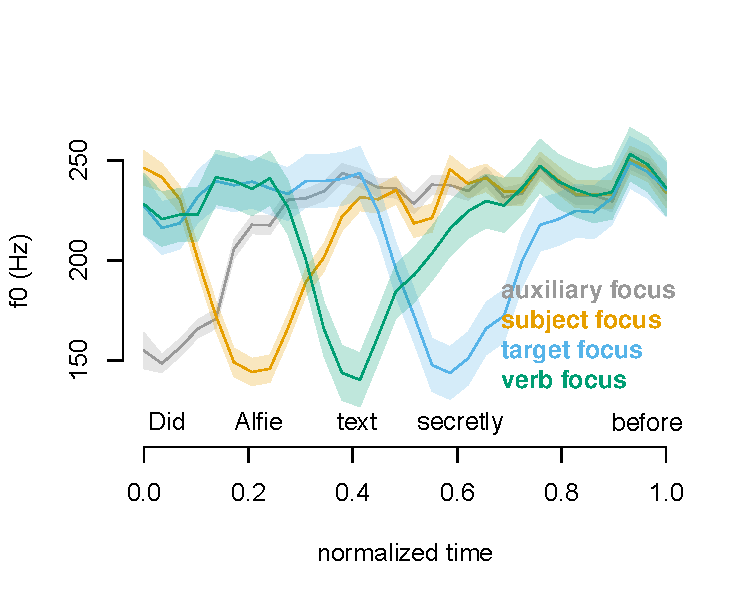
\includegraphics[width=.4\paperwidth]{/Users/tonhauser.1/Documents/current-research-topics/NSF-NAI/prop-att-experiments/8-stop-again-manner/paper/pictures/GAMM-manner-raw}
\caption{Stimuli with manner adverbs}
\end{subfigure}\hspace*{1.5cm}
\begin{subfigure}{.4\textwidth}
\centering
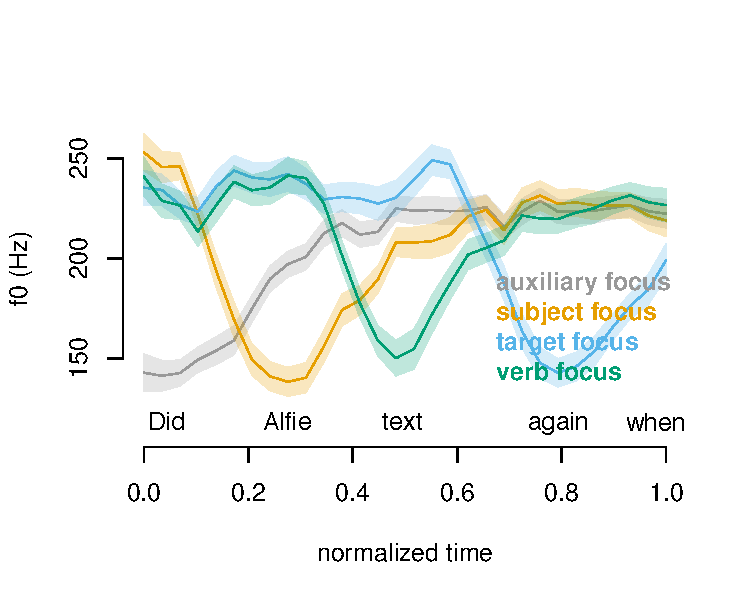
\includegraphics[width=.4\paperwidth]{/Users/tonhauser.1/Documents/current-research-topics/NSF-NAI/prop-att-experiments/8-stop-again-manner/paper/pictures/GAMM-again-raw}
\caption{Stimuli with {\em again}}
\end{subfigure} 

\vspace*{-1cm}

\begin{subfigure}{1\textwidth}
\centering
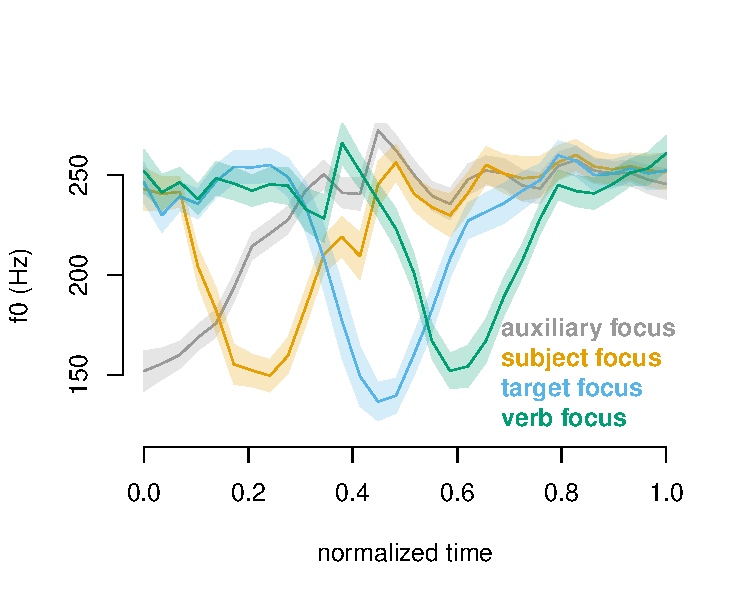
\includegraphics[width=.43\paperwidth]{/Users/tonhauser.1/Documents/current-research-topics/NSF-NAI/prop-att-experiments/8-stop-again-manner/paper/pictures/GAMM-stop-raw}
\caption{Stimuli with {\em stop}}
\end{subfigure}

\caption{Non-linear smooths of the fitted f0 values for the main clauses and temporal adjunct markers of the target stimuli, by focus condition. Shaded bands indicate pointwise 95\% confidence intervals.}\label{f-gamm}
\end{figure}

The 432 utterances were divided into 12 lists of 36 target stimuli so that each list realized each of the 12 main clause verbs with each of its 3 adjunct clauses (i.e., a total of 36 distinct combinations of main clause verbs and adjunct clauses). Both the factor `target expression' (with 3 levels: {\em again, stop}, manner adverb) and the factor `focus condition' (with 4 levels: auxiliary, subject, verb, target) were fully crossed on each list according to a latin square design. In addition to the 36 target stimuli, each list realized 4 control stimuli, which were productions of the 4 polar questions with {\em after-}clauses in (\ref{controls}). These control stimuli were included to assess whether participants were attending to the task and interpreted the task correctly. We expected their main clause contents to be not projective: for instance, we expected the content that Sue came over to not project from (\ref{controls}a). 

\begin{exe}
\ex\label{controls} 
\begin{xlist}

\ex Did Sue come over after Paul left?

\ex Did Gina send an email after the meeting ended?

\ex Did Frank go to Cancun after he graduated?

\ex Did Mark watch TV after he got home?

\end{xlist}
\end{exe}

The 40 stimuli were realized on each list in a pseudo-randomized order.

\subsection{Procedure}

Participants were randomly assigned to a list and told to imagine that they are at a party and that, upon walking into the kitchen, they overhear Debby, the party host, ask another guest a question. They were presented with the 40 stimuli, one after the other. On each trial, participants listened to the stimulus as often as they wanted and then responded to the `certain that' question on a 5-point Likert scale labeled `No, Debby is not certain' (coded as 1) at one end and `Yes, Debby is certain' (coded as 5) at the other end, as shown in Figure \ref{f-trial}. 


\begin{figure}[h!]
\centering

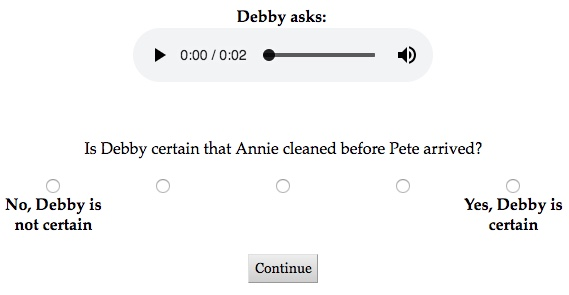
\includegraphics[width=9.5cm]{/Users/tonhauser.1/Documents/current-research-topics/NSF-NAI/prop-att-experiments/8-stop-again-manner/paper/pictures/trial} 


\caption{A sample trial}\label{f-trial}
\end{figure}

Participants then filled out a brief questionnaire about their age, their gender, their native language(s) and, if English is a native language, whether it is American English, as opposed to, e.g., Indian or Australian English. They were told that they would be paid no matter how they responded to these questions, to encourage them to answer truthfully.

\subsection{Data exclusion}

Prior to analysis, we excluded the data of 5 participants who did not self-identify as native speakers of American English. Of the remaining 171 participants, 6 selected `No, Debby is not certain' in all 40 trials; we also excluded their data under the assumption that they did not attend to the task or interpreted the task differently. The remaining 165 participants gave low responses to the 4 control stimuli: as shown in the left panel of Figure \ref{f-control-histogram}, most responses were 1 or 2 (the group mean response was 1.7). For 126 of the 165 participants, the mean response to the 4 control stimuli was at or below 2, as shown in the right panel of Figure \ref{f-control-histogram}.

\begin{figure}[h!]

\begin{subfigure}{.5\textwidth}
\centering
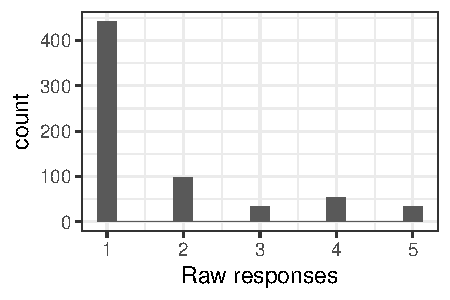
\includegraphics[width=.35\paperwidth]{/Users/tonhauser.1/Documents/current-research-topics/NSF-NAI/prop-att-experiments/8-stop-again-manner/results/graphs/controls-histogram}
%\caption{Inference diagnostic for entailment}
\end{subfigure}%
\begin{subfigure}{.5\textwidth}
\centering
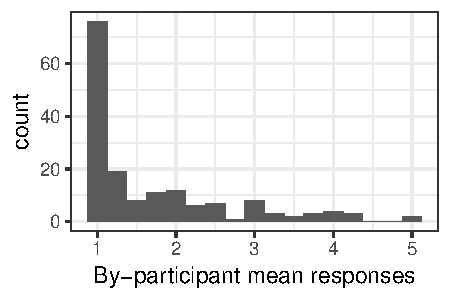
\includegraphics[width=.35\paperwidth]{/Users/tonhauser.1/Documents/current-research-topics/NSF-NAI/prop-att-experiments/8-stop-again-manner/results/graphs/controls-mean-histogram}
%\caption{Contradictoriness diagnostic for entailment}
\end{subfigure}

\caption{Histogram of 165 participants' raw responses (left panel) and mean responses (right panel) to the 4 control stimuli.}\label{f-control-histogram}
\end{figure}

 The results presented in the next section are based on the data from the 126 participants for whom the content of the controls on average was not projective (ages 21-76; mean age: 36; 62 women, 64 men).\footnote{There are no substantial changes to the findings we report on in the next section if the data from the 39 participants with higher mean certainty ratings on the control stimuli are included in the analyses; see footnote \ref{fn}.} 
 The group mean response to the 4 controls by these participants was 1.2.

\section{Results}\label{s3}

We start by addressing the question of how projective the three contents are. The box plot in Figure \ref{f-projectivity} shows the certainty ratings for the contents by expression, collapsing over focus conditions and lexical contents, as well as the certainty ratings for the control stimuli. The mean certainty ratings are given by larger black dots, the notches indicate medians and the smaller black dots indicate outliers. The raw ratings are given by jittered transparent dots: each of the 432 target polar questions received between 5 and 16 certainty ratings (mean: 10.5); there are 1,512 ratings for each projective content and 504 for the contents of the controls. As expected, the mean certainty rating for target stimuli with manner adverbs was low (1.8), suggesting weak projectivity of the prejacent of manner adverbs; the median certainty rating was 1. For target stimuli with {\em again}, neither the mean certainty rating (3.7) nor the median certainty rating (4) were at ceiling, contrary to the predictions of lexicalist analyses of the prejacent of {\em again}. The mean certainty rating for the pre-state content of {\em stop} (3.8) was numerically the highest of the three projective contents investigated; here, the median certainty rating (5) was at ceiling.

\begin{figure}[h!]
\centering

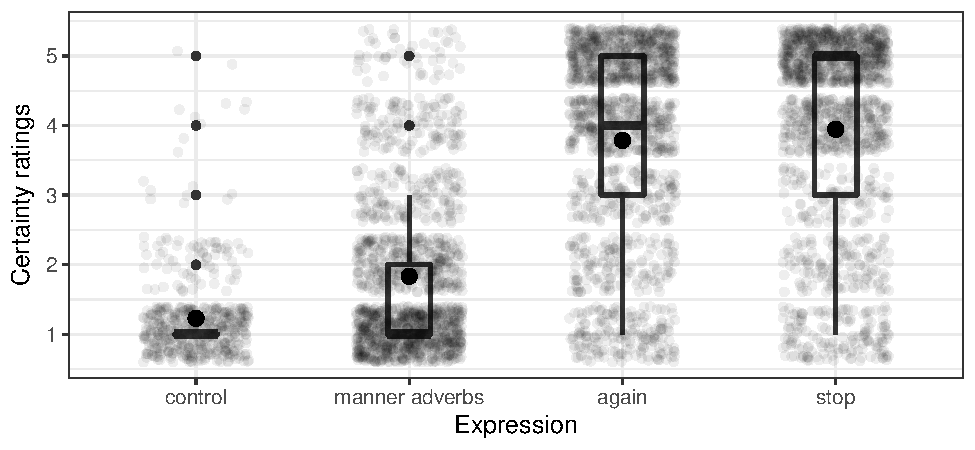
\includegraphics[width=.6\paperwidth]{/Users/tonhauser.1/Documents/current-research-topics/NSF-NAI/prop-att-experiments/8-stop-again-manner/results/graphs/boxplot-projection-with-controls}

\caption{Box plot of certainty ratings by expression, collapsing over focus conditions and lexical contents, as well as of the controls. Larger black dots indicate means, notches indicate medians and smaller black dots indicate outliers. Raw certainty ratings are represented by jittered transparent dots.}
\label{f-projectivity}
\end{figure}

To compare the projectivity of the three contents to each other and to the non-projecting controls, we fitted an ordinal mixed effects model predicting the certainty ratings from a fixed effect of expression (with `control' as the reference level and treatment coding), using the \verb|ordinal| package (version 2018.4-19, \citealt{Christensen2013}) in R (version 3.5.0, \citealt{r}; 5,040 data points). The model included the maximal random effects structure justified by the data and the theoretical assumptions that allowed the model to converge: random by-verb intercepts (capturing differences in projectivity between verbs), random by-lexical content intercepts (capturing differences in projectivity between the lexical contents of the  subjects and adjunct clauses), random by-item intercepts (capturing differences in projectivity between items), random by-participant intercepts (capturing differences in projectivity between participants) and random slopes for expression by participant (capturing that the effect of expression may vary across participants). We then conducted a pairwise comparison with the \verb|lsmeans| package (\citealt{tukey}, version 2.27-62) using Tukey's correction for multiple comparisons.

Compared to the ratings for the non-projective content of the controls, the ratings were significantly higher for the prejacent of manner adverbs ($\beta$ = 1.82, $SE$ = 0.4, $z$ = 4.58, $p <$ .0001), for the prejacent of {\em again} ($\beta$ = 5.89, $SE$ = 0.48, $z$ = 12.23, $p <$ .0001) and for the pre-state content of {\em stop} ($\beta$ = 6.38, $SE$ = 0.49, $z$ = 12.93, $p <$ .0001). These findings confirm that the three contents under investigation are projective. Furthermore, certainty ratings for the prejacent of {\em again} were lower than those for the pre-state content of {\em stop} ($\beta$ = -.49, $SE$ = 0.14, $z$ = -3.45, $p =$ .0032), and ratings for the prejacent of manner adverbs were lower than those for the prejacent of {\em again} ($\beta$ = -4.07, $SE$ = 0.31, $z$ = -13.06, $p <$ .0001) and for the pre-state content of {\em stop} ($\beta$ = -4.56 $SE$ = 0.34, $z$ = -13.45, $p <$ .0001). In sum, the prejacent of manner adverbs is projective, albeit only weakly so compared to the prejacent of {\em again} and the pre-state content of {\em stop}. Furthermore, the projectivity of the prejacent of {\em again} was lower than that of the pre-state content of {\em stop} and, contrary to expectation, not at ceiling. 

We next address the question of whether projectivity is sensitive to information structural focus by assessing whether certainty ratings are sensitive to the prosodic manipulation. The box plot in Figure \ref{f-projectivity2} shows the certainty ratings for the projective contents by expression and focus condition, collapsing over lexical contents. As above, the mean certainty ratings are given by larger black dots, the notches indicate medians and the smaller black dots indicate outliers. The raw certainty ratings are given by jittered transparent dots: there are 378 ratings per projective content in each of the four focus conditions. As expected, both the mean and the median certainty ratings for the prejacent of manner adverbs are higher in the target condition (where the L* pitch accent was realized on the manner adverb) than in the other three focus conditions. The same pattern is observed for the prejacent of {\em again}: both the mean and the median certainty ratings are higher in the target condition (L* pitch accent on {\em again}) than in the other three focus conditions. For the pre-state content of {\em stop}, the mean certainty rating is also highest in the target condition (L* pitch accent on {\em stop}); here, the median certainty rating is higher in the target and verb conditions than in the auxiliary and subject conditions. 

\begin{figure}[h!]
\centering

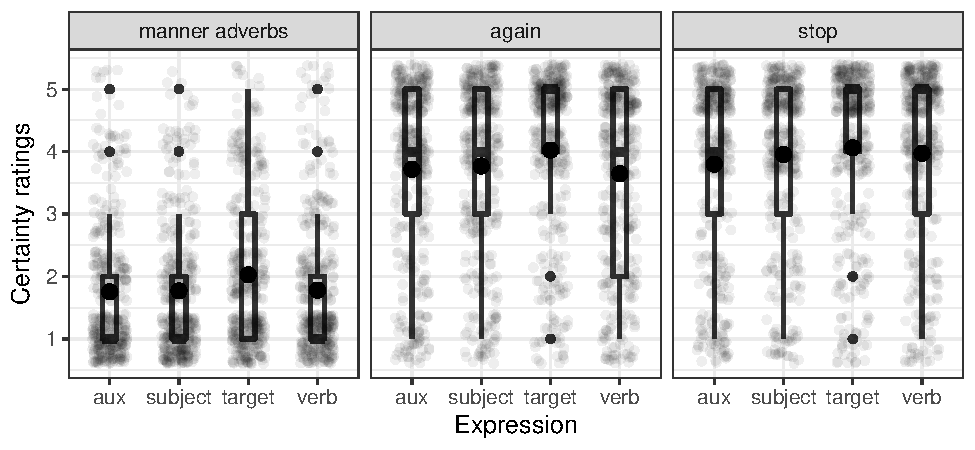
\includegraphics[width=.65\paperwidth]{/Users/tonhauser.1/Documents/current-research-topics/NSF-NAI/prop-att-experiments/8-stop-again-manner/results/graphs/boxplot-projection-by-prosody}

\caption{Box plot of certainty ratings by target expression and focus condition, collapsing over lexical contents. Larger black dots indicate means, notches indicate medians and smaller black dots indicate outliers. Raw certainty ratings are represented by jittered transparent dots.}
\label{f-projectivity2}
\end{figure}


To assess the influence of focus condition on the certainty ratings, we fitted ordinal mixed effects models predicting the ratings from focus condition (with `target' as the reference level and treatment coding); we built a separate model for each content (1,512 data points each).  The three models included the same random effects structure as the aforementioned model. We then conducted pairwise comparisons of the focus conditions using the \verb|lsmeans| package, as above.

For the prejacent of manner adverbs, the certainty ratings in the target condition were significantly higher than those in the auxiliary condition ($\beta$ = .87, $SE$ = 0.23, $z$ = 3.75, $p = $ .001), the subject condition ($\beta$ = .71, $SE$ = 0.19, $z$ = 3.68, $p = $ .0013) and the verb condition ($\beta$ = .68, $SE$ = 0.18, $z$ = 3.69, $p = $ .0013).\footnote{A model that was identical except that it included the non-projective contents of the controls showed that the prejacent of manner adverbs received significantly higher certainty ratings than the content of the controls in each of the focus conditions. This finding suggests that the prejacent is projective in each of the focus conditions.} Likewise for the prejacent of {\em again}: the certainty ratings in the target condition were significantly higher than those in the auxiliary condition ($\beta$ = .74, $SE$ = 0.19, $z$ = -4, $p = $ .0004), the subject condition ($\beta$ = .52, $SE$ = 0.19, $z$ = 2.72, $p = $ .03) and the verb condition ($\beta$ = .78, $SE$ = 0.19, $z$ = 4.13, $p = $ .0002). For the pre-state content of {\em stop}, the certainty ratings in the target condition were significantly higher than those in the auxiliary condition ($\beta$ = .7, $SE$ = 0.19, $z$ = 3.6, $p = $ .0017) and marginally higher than those in the subject condition ($\beta$ = .46, $SE$ = 0.19, $z$ = 2.37, $p = $ .08); the certainty ratings in the auxiliary condition were marginally lower than those in the verb condition ($\beta$ = -.5, $SE$ = 0.2, $z$ = -2.49, $p = $ .06).\footnote{\label{fn}A model that was fit on the data that included the data from the 39 participants with higher mean certainty ratings on the control stimuli showed that the certainty ratings in the auxiliary condition for {\em stop} were significantly lower than those in the verb condition ($\beta$ = -.41, $SE$ = 0.15, $z$ = -2.72, $p < $ .05).} No other pairwise comparisons were significant. 

These findings suggest that the projectivity of the three projective contents investigated is sensitive to prosodically marked information structural focus. The three contents differed, however, in how the prosodic manipulation affected the certainty ratings. For manner adverbs and {\em again}, the prejacent was more projective when the L* pitch accent was realized on the manner adverb or on {\em again}, respectively, than when the L* pitch accent was realized on the auxiliary, the subject or the verb. For {\em stop}, the pre-state content was more projective when the L* pitch accent was realized on {\em stop} than when it was realized on the auxiliary.

\section{Discussion}\label{s4}

The experiment reported on in this paper was designed to investigate the projectivity of the prejacent of manner adverbs, the prejacent of {\em again} and the pre-state content of {\em stop}, as well as whether their projectivity is sensitive to prosodically marked information structural focus. In this section, we discuss whether current analyses account for our findings (sections \ref{s41} to \ref{s43}) and also discuss implications for empirically adequate projection analyses (section \ref{s44}).

\subsection{Prejacent of manner adverbs}\label{s41}

As discussed in section \ref{s1}, the projectivity of the prejacent of manner adverbs is generally attributed to information structural focus (e.g., \citealt{abrusan2013,stevens-etal2017}); specifically, these analyses predict that if the manner adverb is in focus, the prejacent is projective. This prediction is supported by our experiment findings: the prejacent of manner adverbs was projective when the L* pitch accent was realized on the manner adverb, i.e., when the prosodic realization of the polar question provided a cue to the manner adverb being in focus. A second finding that projection analyses need to account for is that the prejacent was only weakly projective. As discussed in section \ref{s1}, \citet{stevens-etal2017} assumed that the prejacent projects if it is entailed by the QUD addressed by the utterance, with the QUD constrained by information structural focus, among other things. Taken together with the assumption that prosody provides a cue to, but does not determine, information structural focus (see, e.g., \citealt{breen-etal10,tonhauser-prosody}),  we hypothesize that the prejacent of manner adverbs was only weakly projective when the L* pitch accent was realized on the manner adverb because listeners may have uncertainty about i) whether the manner adverb was in focus, and ii) whether the speaker's utterance was relevant to a QUD that entailed the prejacent. 

This hypothesis leads us to expect higher certainty ratings when there is less uncertainty about what is focused or about the QUD. An interesting test case is a language like Hungarian in which what is focused is syntactically constrained (e.g., \citealt{szabolcsi81,kiss87}). As discussed in \citealt{abrusan2013}, the preverbal expression is focused in Hungarian when the aspectual particle of the verb appears after the verb. Thus, the manner adverb {\em hangosan} `loudly' is not focused  in (\ref{hung}a), but it is focused in (\ref{hung}b), where the particle {\em el} appears after the verb. 

\begin{exe}
\ex\label{hung} Hungarian, adapted from \citealt[260]{abrusan2013}
\begin{xlist}

\ex \gll K\'etlem, hogy P\'eter hangosan el\'enekelte a Himnuszt \\ doubt.1sg that Peter loudly prt.sang the anthem.acc \\ \glt `I doubt that Peter sang the anthem loudly.' 

\ex \gll K\'etlem, hogy P\'eter hangosan \'enekelte el a Himnuszt \\ doubt.1sg that Peter loudly sang prt the anthem.acc \\ \glt `I doubt that Peter sang the anthem loudly.'  

\end{xlist}
\end{exe}
According to \citet[260]{abrusan2013}, the prejacent, that Peter sang the anthem, projects in (\ref{hung}b) but not in (\ref{hung}a). Whether the prejacent of manner adverbs is more projective when what is focused is syntactically marked (as in the Hungarian examples above) than when it is only prosodically cued (as in our English stimuli) is an open question for future research. 

A third finding that projection analyses need to account for is that the prejacent was weakly projective even when the L* pitch accent  was realized on an expression other than the manner adverb. This finding is incompatible with the assumption made in, for instance, \citealt{simons01} and \citealt{abrusan2013}, that the prejacent is not projective when an expression other than the manner adverb is in focus. This assumption is not made in \citealt{stevens-etal2017}: here, the prejacent is predicted to project if it is entailed by the QUD (note the {\em if}!), which leaves open the possibility of other factors contributing to the projectivity of the prejacent. 

One possibility is that the projectivity of the prejacent, i.e., the inference that the speaker is committed to the truth of the prejacent, is a conversational implicature. To illustrate, consider the pair of polar questions in (\ref{iron}). 

\begin{exe}
\ex\label{iron} 
\begin{xlist}
\ex Was Sandy smiling?

\ex Was Sandy smiling ironically?
\end{xlist}
\end{exe}
The polar question in (\ref{iron}a) is appropriate when the issue of whether Sandy was smiling is open, i.e., the speaker's epistemic state is compatible with Sandy having smiled and with Sandy not having smiled. In fact, this is an open issue even if one of the three expressions in (\ref{iron}a) is focused. Now consider an utterance of the variant with the manner adverb in (\ref{iron}b). Given that the speaker could have uttered the simpler polar question in (\ref{iron}a), listeners will assume that a speaker who utters (\ref{iron}b) is not merely interested in resolving the issue of whether Sandy was smiling. Rather, listeners may assume that such a speaker is interested in resolving a more specific issue. With focus on the auxiliary or the manner adverb, that more specific issue appears to be whether the manner in which Sandy was smiling was ironic, which implies that the speaker already assumed that Sandy was smiling. With focus on the subject proper name, the more specific issue appears to be who the individuals are who were smiling ironically. Given that only individuals who were smiling are relevant and given that Sandy was mentioned as a possible alternative, listeners may take the speaker to be committed to Sandy having smiled. Finally, with focus on the participle {\em smiling}, the more specific issue appears to be which activity Sandy was engaged in in an ironic manner. Again, the listener may assume that the speaker is only considering activities  that Sandy is already engaged in and therefore that Sandy was smiling. In short, the prejacent of (\ref{iron}b) may be projective as a result of listeners' reasoning about speakers' epistemic states and alternative polar questions that speakers could have uttered.

In sum, our experiment found that the prejacent of manner adverbs is weakly projective regardless of focus condition and that it is more projective when the manner adverb is focused. These findings are accounted for by \citetpos{stevens-etal2017} focus-based analysis in combination with domain-general reasoning about speakers' utterances. 

\subsection{Prejacent of {\em again}}\label{s42}

As discussed in section \ref{s1}, the projectivity of the prejacent of {\em again} is generally accounted for by specifying it as a presupposition in the lexical entry of {\em again} (e.g., \citealt{kamp-rossdeutscher1994,fabricius-hansen2001,simons01,jaeger-blutner2003,vds-huitink2003,beck2006}; but see \citealt{abrusan2013b,abrusan2016}). As a lexically specified presupposition, we expect the prejacent to be highly projective, even more so because {\em again} is typically considered a `hard' trigger. However, contrary expectation, the mean certainty rating for the prejacent of {\em again} was only 3.7 (out of 5) and the median certainty rating (4) was also not at ceiling.\footnote{Our assumption that the observed certainty ratings for the prejacent of {\em again} are lower than ceiling is also justified by the finding that the certainty ratings for the pre-state content of {\em stop} were significantly higher.}

This finding differs from that of \citealt{xue-onea11} for German {\em wieder} `again'.  There are, however, several important differences between the two experiments, including the entailment-canceling environment (antecedent of conditional in \citealt{xue-onea11}  vs.\ polar question in ours), the response task (possibility of prejacent being false vs.\ certainty ratings), the response options offered to the participants (`yes, it's possible'/`no, it's not possible'/`I don't know' vs.\ 5-point Likert scale), the other projective contents explored, the presentation of the stimuli (in writing vs.\ auditorily), the number of participants (34 vs.\ 126), the number of  items judged by each participant (3 vs.\ 12),  as well as whether prosody was manipulated. Future research will need to establish whether (a combination of) any of these differences contributed to the different finding or whether there is cross-linguistic variation.
 
Do currently available projection analyses predict our findings for the prejacent of {\em again}? We first consider analyses of the prejacent as a lexically specified presupposition. Such analyses generally rely on the process of local accommodation to account for non-projecting presuppositions: local accommodation is typically assumed for presuppositions that need to be accommodated (i.e., that are not in the common ground of the interlocutors when the sentence with the triggering expression is uttered) and for which the default global accommodation would lead to contradiction with information already in the common ground, uninformativity or problems with binding (e.g., \citealt{heim83,vds92}). In our experiment, default global accommodation cannot be assumed to be overridden by information contributed by prior utterances. However, as discussed in \citealt{djaerv-bacovcin-salt27} for utterances of sentences with factive predicates like {\em discover}, the prosodic realization of the utterance may contribute an inference that contradicts the presupposition, thereby resulting in local accommodation. To illustrate \citetpos{djaerv-bacovcin-salt27} proposal, consider an utterance of the sentence with the factive predicate {\em discover} in (\ref{db}) in which the subject of the clausal complement, {\em Anna}, is focused, as indicated by the brackets with the subscripted `F'.

\begin{exe}
\ex\label{db} John might have discovered that [Anna]$_{\mbox{F}}$ left town. \hfill (\citealt[129]{djaerv-bacovcin-salt27})
\end{exe}
Under a lexicalist analysis, the content of the complement of {\em discover}  is lexically specified as a presupposition. As a consequence, if the content of the complement in (\ref{db}), that Anna left town, is not part of the common ground at the time at which (\ref{db}) is uttered, it must be accommodated, with global accommodation being the default. \citet{djaerv-bacovcin-salt27} suggested that focus on {\em Anna} implies that the QUD addressed by (\ref{db}) is something like `Who left town?', which implies that the speaker does not know whether Anna left town. \citet{djaerv-bacovcin-salt27} proposed that there is an interaction between the lexically specified presupposition and the inference from focus: listeners are less likely to globally accommodate the presupposed content of the complement because doing so would contradict the inference contributed by focus.

This kind of account does not, however, seem to be able to predict local accommodation of the presupposed prejacent of {\em again}. Consider the sentence in (\ref{again}b), repeated below for convenience, in which {\em again}, according to a lexicalist analysis, triggers the presupposition that Sam visited Barcelona before July 2018. In order for the QUD addressed by (\ref{again}b) to override the default global accommodation of this presupposition, the QUD would need to imply that the speaker does not know whether Sam visited Barcelona before early July 2018.  

\begin{exe}
\exi{(\ref{again}b)} Did Sam visit Barcelona again in early July 2018?
\end{exe}
It does not appear to be the case that focus on any of the expressions in this polar question yields such a QUD. Consider, for instance, focus on {\em Sam}: (\ref{again}b) may then be taken to be part of a discourse in which the QUD is something like `Who visited Barcelona in early July 2018?'.\footnote{Following \citealt[fn.4]{beck2006}, we assume that {\em again} contributes only presupposed material and that, therefore, its contribution is not part of the focus-induced alternatives.} This QUD implies uncertainty on part of the speaker about who visited Barcelona in early July 2018, but not about whether Sam visited Barcelona before July 2018. What if {\em again} is focused in (\ref{again}b)? \citet[\S5]{beck2006} assumed that the alternatives to {\em again} are an empty adverb and {\em still}. Thus, if {\em again} is focused in (\ref{again}b), the QUD addressed by (\ref{again}b) is something like the set \{Sam visited Barcelona again in early July 2018, Sam visited Barcelona in early July 2018, Sam is still visiting Barcelona in early July 2018\}. This semantic question implies that the speaker knows that Sam visited Barcelona in early July 2018, but not whether Sam's visit in Barcelona began at a time before July 2018 and has continued to early July 2018, or whether Sam went elsewhere in the mean time. Crucially, however, because this QUD does not imply that the speaker does not know whether Sam visited Barcelona before early July 2018, focus on {\em again} does not override the default global accommodation of the presupposed prejacent. 

On Abrus\'an's (2013b; 2016) account, the prejacent of {\em again} is projective not because it is a lexically specified presupposition but because it is an entailment that is by default backgrounded. Although Abrus\'an's account allows for the possibility of entailments that are by default backgrounded to be foregrounded and therefore not projective (for instance when the QUD is about the entailed content), Abrus\'an also assumed that the prejacent of {\em again} (as well as that of other additive particles) cannot be suspended (\citealt[e.g., 167, 168, \S2.2]{abrusan2016}). Consequently, her account is designed to predict that the prejacent of {\em again} cannot be suspended, regardless of which expression is focused, and it therefore does not account for our experiment findings. In sum, current analyses of the prejacent of {\em again} do not account for the lower-than-ceiling certainty ratings observed for {\em again} in our experiment.


Our finding that the projectivity of the prejacent of {\em again} is not at ceiling resonates with the observation, reported in \citealt[fn.3]{abrusan2016}, that suspension examples like (\ref{suspend}a), repeated below, may not be judged to be as unacceptable as parallel examples with other supposedly `hard' presupposition triggers, like {\em too}. 

\begin{exe}
\exi{(\ref{suspend}a)} {[}The speaker observes Jane, whose history of video rental she knows nothing about, in a video store.] \\ \infelic I have no idea whether Jane ever rented ``Manhattan'', but perhaps she is renting it again. \\ \hspace*{.2cm} \hfill (\citealt[433]{simons01})
\end{exe}
This kind of observation, together with our experiment findings, suggest that it is not empirically adequate to classify {\em again} as a `hard' presupposition trigger. 

Recall that our experiment also found that the projectivity of the prejacent of {\em again} was sensitive to the prosodic manipulation of information structural focus: the prejacent was more projective when the L* pitch accent was realized on {\em again} than when the L* pitch accent was realized on another expression in the main clause. Neither the lexicalist analysis nor Abrus\'an's entailment-based analysis of the projectivity of the prejacent accounts for the observed sensitivity to information structural focus (under the assumption that the expression that realizes the L* pitch accent is in focus). The lexicalist analysis does not because, as discussed above, focus on any of the expressions in the main clause does not lead to QUDs that would override the default global accommodation. And on Abrus\'an's account, too, the projectivity of the prejacent of {\em again} is, by design, independent of information structural focus. 

Before concluding this section, we consider a different avenue for accounting for the sensitivity of the projectivity of the prejacent of {\em again} to the prosodic manipulation. This consideration is based on the long-standing observation that {\em again} is compatible not only with the repetitive interpretation entertained thus far, but also with a so-called restitutive interpretation. Crucially, focus on {\em again} decreases the availability of the restitutive interpretation. To illustrate, consider the examples in (\ref{open}). The example in (\ref{open}a), with focus on {\em opened}, can receive both a repetitive interpretation (Otto had opened the door before, and now he opened it again) and a restitutive interpretation (somebody had closed the door, and Otto has caused it to be open again). By contrast, (\ref{open}b), with focus on {\em again}, is biased towards a repetitive interpretation. 

\begin{exe}
\ex\label{open} \citealt[280]{beck2006}
\begin{xlist}

\ex Otto OPENED the door again.

\ex Otto opened the door AGAIN.

\end{xlist}
\end{exe}
Restitutive {\em again} does not give rise to the inference under consideration in this paper: under a restitutive interpretation, (\ref{open}a) does not imply that Otto opened the door before. Is it possible that our experiment found higher certainty ratings for stimuli in which the L* pitch accent was realized on {\em again} because these stimuli favor a repetitive interpretation? We argue that this is not a possible explanation for our findings. The restitutive interpretation is only available for predicates that describe an event with a result state: with such predicates, {\em again} can contribute the information that the result state was restored. As discussed in section \ref{s2}, the predicates in our stimuli were {\em text, clean, shout, yell, bark, knock, whistle, speak, walk, smile, cry} and {\em giggle} in their intransitive frames. Except for {\em clean}, none of these predicates have telic uses (e.g., {\em Sam whistled for/*in 2 hours}, but {\em Sam cleaned for/in 2 hours}), which means that they are incompatible with a restitutive interpretation. However, even though the restitutive interpretation is possible for {\em clean}, the effect of focus condition on the projectivity of the prejacent of {\em again} was not limited to stimuli with {\em clean} (recall that the model we fit to the data in section \ref{s3} included a by-verb intercept). Thus, the lower-than-ceiling projectivity of the prejacent of {\em again} cannot be attributed to the restitutive interpretation of {\em again}.

In sum, currently available analyses of the prejacent of {\em again} predict that its projectivity is at ceiling and insensitive to information structural focus. Our experiment findings suggest that both of these predictions are empirically inadequate.

\subsection{Pre-state content of {\em stop}}\label{s43}

As mentioned in section \ref{s1}, the pre-state content of {\em stop} has traditionally been analyzed as a lexically specified presupposition, like the prejacent of {\em again} (e.g., \citealt{heim83,vds92,kadmon01}). Can this type of analysis account for the findings of our experiment? Recall from section \ref{s42} that lexicalist analyses rely on local accommodation to account for non-projecting presuppositions and that the default global accommodation cannot be assumed to be overridden in our experiment by information contributed by prior utterances. Focus-induced inferences about the QUD, however, may conflict with the lexically specified presupposition of {\em stop}, thereby predicting local accommodation. To illustrate, consider the sentence in (\ref{stop}), in which {\em stop}, according to a lexicalist analysis, triggers the presupposition that Sam smoked before he turned 18. In order for the QUD addressed by (\ref{stop}) to override the default global accommodation of this presupposition, the QUD would need to imply that the speaker does not know whether Sam smoked before he turned 18.

\begin{exe}
\ex\label{stop} Did Sam stop smoking when he turned 18?
\end{exe} 
Consider an utterance of (\ref{stop}) with focus on {\em Sam}, which may be taken to be part of a discourse in which the QUD is something like `Who stopped smoking when they turned 18?'. It is possible for such an utterance of (\ref{stop}) to be part of a discourse in which the contextually salient alternatives to {\em Sam} are individuals who used to smoke. In this case there is no uncertainty on part of the interlocutors about whether Sam smoked before he turned 18, i.e., no local accommodation is expected. But it may also be possible for an utterance of (\ref{stop}) with focus on {\em Sam} to be part of a discourse in which the contextually salient alternatives to {\em Sam} include individuals who used to smoke as well as individuals who have never smoked. If so, the listener may take the speaker of (\ref{stop}) to be uncertain about whether Sam smoked before he turned 18. This focus-induced inference about the QUD may then override the default global accommodation of the lexically specified presupposition of {\em stop}, predicting non-projection. 

What about the second finding of our experiment, that the pre-state content is more projective with focus on {\em stop} than with focus on the auxiliary? Whether this finding can be accounted for under a lexicalist analysis depends on i) which alternatives to {\em stop} are considered and ii) and the details of the analysis of focus on the auxiliary, also known as verum focus (e.g., \citealt{hoehle1992}). With respect to i), under a standard focus semantics (e.g., \citealt{rooth92}), the alternatives to {\em stop} are expressions of the same type as {\em stop}, such as {\em continue} or {\em start}. Of course, (\ref{stop}) with focus on {\em stop} may be part of a discourse in which only individuals who smoked before they turned 18 are under consideration. In this case, the alternatives to {\em stop} may be restricted to, for instance {\em continue} and {\em used to}, resulting in a QUD that does not convey uncertainty on part of the speaker about whether Sam smoked before he turned 18. In this case, the presupposition is not predicted to be locally accommodated. But (\ref{stop}) with focus on {\em stop} may also be part of a discourse in which the speaker doesn't know whether Sam smoked before he turned 18. Here the alternatives to {\em stop} might include {\em continue} and {\em start}, in which case the QUD is something like `Has Sam smoked in the past or, if he has, does he still smoke?'. This focus-induced QUD may lead the listener to infer that the speaker is not certain about whether Sam smoked before he turned 18, predicting non-projection. Thus, without further restrictions on the alternatives to {\em stop}, focus on {\em stop} may result in the inference that the speaker is not certain about the presupposed pre-state, resulting in non-projection of the presupposition.

With respect to ii), we consider the analyses of verum focus proposed in \citealt{romero-han2004} and \citealt{gutzmann-miro2011}. Under \citetpos{romero-han2004} proposal, (\ref{stop}) with focus on the auxiliary would denote the question \{$p$: the speaker is sure that Sam stopped smoking when he turned 18, $\neg p$: the speaker is not sure that Sam stopped smoking when he turned 18\}. Because the proposition $\neg p$ can include worlds in which Sam never smoked, a speaker who utters (\ref{stop}) with focus on the auxiliary may be taken to be uncertain about whether Sam smoked before he turned 18, resulting in non-projection of the presupposed pre-state content. Under \citetpos{gutzmann-miro2011} proposal, the positive polar question in (\ref{stop}) with focus on the auxiliary denotes the usual set of alternatives, i.e., \{$p$: Sam stopped smoking when he turned 18, $\neg$$p$: Sam didn't stop smoking when he turned 18\}. Verum focus contributes the use-conditional meaning that the speaker wants to downdate the question: this means that the speaker conveys that (they assume that) the listener is sure that their answer should be added to the common ground (p.162).  Crucially, however, the speaker is not sure about $p$ (otherwise they wouldn't have asked the question), which means that a speaker who utters (\ref{stop}) with focus on the auxiliary may be taken to convey uncertainty about whether Sam smoked before he turned 18, resulting in non-projection of the presupposed pre-state content. In sum, a lexicalist analysis of the pre-state content of {\em stop}, augmented with assumptions about focus alternatives to {\em stop} and an analysis of verum focus, predicts the possibility of non-projection of this content both if {\em stop} is focused and if the auxiliary is focused. It is therefore not clear that such an analysis accounts for the second finding of our experiment, that the pre-state content is more projective with focus on {\em stop} than with focus on the auxiliary.

Non-lexicalist analyses of the pre-state content of {\em stop} (e.g., \citealt{abusch02,abusch10,abrusan2011,abrusan2016,romoli2011,romoli2015,brst-ar}) were driven by two observations. The first one is that this content can be suspended in explicit ignorance contexts, as in (\ref{stop-ei}). This means that {\em stop} is not a `hard' presupposition trigger (but see \citealt{abrusan2016}). In line with this observation, \citealt{tbd-variability} found that the projectivity of the pre-state content of {\em stop} is not at ceiling.

\begin{exe}
\ex\label{stop-ei} I have no idea whether Jane ever smoked, but she hasn't stopped smoking. \\ \hspace*{.2cm} \hfill (\citealt[433]{simons01})
\end{exe}
The second observation is that the pre-state content of {\em stop} does not appear to be associated with the expression but rather with its content; in other words, the pre-state content of {\em stop} is nondetachable (\citealt{grice75}). Evidence comes from \citetpos{simons01} observation that English variants of (\ref{stop-nd}a) with {\em quit, cease} and {\em discontinue} give rise to the same content and \citetpos{brst-lang11} finding that the same is true of the Paraguayan Guaran\'i variant of (\ref{stop-nd}a) in (\ref{stop-pg}): here, the change-of-state meaning is not coded by a lexical item but by the combination of the negation circumfix, the suffix {\em --ve} `more' and perfect aspect  {\em --ma} (see also \citealt{levinson-annamalai92}):\footnote{The glosses in the Paraguayan Guaran\'i examples follow the Leipzig Glossing Conventions, except for `A3', which is a third person marker from the set A series (\citealt{tonhauser-bruno}).}

\begin{exe}
\ex\label{stop-nd} \citealt[435]{simons01}
\begin{xlist}
\ex Jane didn't stop laughing.
\ex Jane didn't quit laughing.
\ex Jane didn't cease laughing. 
\ex Jane did not discontinue her laughter.
\end{xlist}

\ex\label{stop-pg} \gll J\'ane nd-o-puka-v\'e-i-ma. \\ Jane {\sc neg-}A3-laugh-more{\sc -neg-prf} \\ \glt `Jane stopped laughing.' 
\end{exe}

Do non-lexicalist analyses of the pre-state content of {\em stop} predict the findings of our experiment? On Abusch's (2002, 2010) analysis, the projectivity of this content is derived from the assumption that the conventionally specified alternative to {\em stop} is {\em continue} and the assumption that propositions that are entailed by each alternative in the set of alternatives are projective, unless there is contextual evidence to the contrary. For (\ref{stop}), the set of alternatives is \{Sam stopped smoking when he turned 18, Sam continued smoking when he turned 18\}. Because each alternative in this set entails that Sam smoked before he turned 18, the pre-state content is predicted to be projective. To assess whether Abusch's (2002, 2010) analysis accounts for the findings of our experiment, let's assume that focus-induced inferences about the QUD can provide evidence that the speaker is not committed to the pre-state content, and thereby provide contextual evidence about non-projection. Because alternatives to {\em stop} are lexically specified, focus on {\em stop} does not lead the listener to infer that the speaker is not certain about the pre-state content. Thus, Abusch's (2002, 2010) analysis does not appear to predict lower-than-ceiling ratings when {\em stop} is focused. However, given that verum focus can lead to non-projection, Abusch's (2002, 2010) analysis correctly predicts that projectivity is lower when the auxiliary is focused than when {\em stop} is focused.

On Romoli's (2011, 2015) analysis, the projectivity of the pre-state content of {\em stop} is derived as a scalar implicature (see also \citealt{chemla09}). Romoli takes the lexically specified alternative of {\em stop} to be {\em used to}: thus, the set of alternatives associated with the sentence {\em Sam stopped smoking when he turned 18} is the set $Alt_1$:\{Sam stopped smoking when he turned 18, Sam used to smoke before he turned 18\}\footnote{It may be better to characterize this alternative as the proposition that Sam smoked before he turned 18, because {\em used to} implies a change of state, but we stick here with Romoli's specification of the alternative.} and the set of alternatives associated with the negated sentence {\em Sam didn't stop smoking when he turned 18} is the set $Alt_2$:\{Sam didn't stop smoking when he turned 18, Sam didn't used to smoke before he turned 18\}. Romoli assumed that scalar implicatures arise as entailments of exhaustified sentences (e.g., \citealt{chierchia-etal2012}) and he also assumed that both answers of a polar question are exhaustified. Consider now the polar question in (\ref{stop}), repeated below for convenience. Under Romoli's analysis, (\ref{stop}) denotes the set of exhaustified alternatives in (\ref{rstop}). Exhausification of the first alternative proposition in (\ref{rstop}) affirms the (positive) proposition $p$ in the scope of the exhaustification operator {\sc exh} and negates those alternatives in $Alt_1$ whose negation is consistent with $p$, i.e., none of the propositions in $Alt_1$ are negated. Exhaustification of the second alternative proposition in (\ref{rstop}) affirms the (negated) proposition $p$ in the scope of the exhaustification operator {\sc exh} and negates those alternatives in $Alt_2$ whose negation is consistent with $p$. Here, exhaustification negates the proposition that Sam didn't used to smoke before he turned 18, i.e., affirms that Sam used to smoke before he turned 18. Because the proposition that Sam used to smoke before he turned 18 follows from both exhaustified alternatives in (\ref{rstop}), the pre-state content is predicted to project.

\begin{exe}
\exi{(\ref{stop})} Did Sam stop smoking when he turned 18?
\ex\label{rstop} \{{\sc exh}[Sam stopped smoking when he turned 18], {\sc exh}[Sam didn't stop smoking when he turned 18]\}
\end{exe}

\citet[201]{romoli2015} assumed that the pre-state content projects ``unless we have information in the context that the speaker is ignorant about it''. Given what we have said above about the possibility of deriving non-projection from information about focus-induced inferences about the QUD, this suggests that Romoli's (2011, 2015) analysis could account for the observed lower-than-ceiling ratings, at least when an expression other than {\em stop} is focused. However \citet[200]{romoli2015} also assumed that the projection of soft presuppositions, including the pre-state content of {\em stop}, cannot be suspended by considerations about whether the pre-state content is relevant to the question under discussion: ``relevance is not taken into account and exhaustification has to always happen on the entire set of alternatives''. This suggests that focused-induced inferences about the question under discussion are predicted to not influence the projectivity of the pre-state content of {\em stop}, contrary to the findings of our experiment. 

On Abrus\'an's (2011, 2016) analysis, entailments that are not about the event time of the matrix predicate are backgrounded and therefore project unless they are ``the most direct answer to the (grammatically signalled) background question'' (\citealt[511]{abrusan2011}). Because focus can induce inferences about the QUD, Abrus\'an's analysis appears to predict that the projectivity of the pre-state content of {\em stop} is not at ceiling. However, \citet{abrusan2016} did not consider how focus could suspend the pre-state content of {\em stop} because she assumed that the pre-state content ``cannot be suspended that easily'' (p.193). This assumption runs contrary to the findings of our experiment and that of \citealt{tbd-variability}, where the pre-state content of {\em stop} was significantly less projective than other presuppositions. As for the second finding of our experiment, it is unclear whether this finding is accounted for under Abrus\'an's analysis, given that focus on both expressions is compatible with non-projection, as discussed above.

The last analysis we consider is the one proposed in \citealt{brst-ar}: here,  the pre-state content projects if and only if it is not at-issue with respect to the QUD (see also \citealt{brst-salt10,tbd-variability}). As with Abrus\'an's analysis, this analysis allows for focus-induced alternatives about the QUD to correctly predict that the projectivity of the pre-state content is not at ceiling. However, this analysis, too, does not appear to predict that the projectivity is lower with focus on the auxiliary than with focus on {\em stop}. In sum, none of the analyses currently on the market correctly predict the findings of our experiment for the pre-state content of {\em stop}. Some analyses correctly predict the first but not the second finding (\citealt{brst-ar,djaerv-bacovcin-salt27}) and others predict the second but not the first one (\citealt{abusch02,abusch10}). A third set of analyses, like that in \citealt{romoli2011,romoli2015}, do not appear to predict either finding. The status of Abrus\'an's (2011, 2016) analysis is unclear, as discussed above.


\subsection{General discussion}\label{s44}

Linguistic research on projective content is driven by the goal of deriving the projectivity of such content from its empirical properties and to account for these properties. Over the past decades, different analyses have been developed for projective contents that differ in their empirical properties: the analysis in \citealt{heim83} was developed for presuppositions, that in \citealt{potts05} for conventional implicatures, and that in \citealt{abrusan2013} for focus-derived projective content. Our understanding of the empirical properties of projective content has been increasing steadily. We now know that the projectivity of utterance content is influenced by a variety of factors, including the meaning of the expression associated with the content (e.g., \citealt{karttunen71b,tbd-variability}), contextual information including perspectival information (e.g., \citealt{gazdar79a,harris-potts09}), information structure (e.g., \citealt{beaver-belly,tonhauser-salt26} and this paper) and at-issueness (e.g., \citealt{tbd-variability}). This increased understanding presents an opportunity to assess projection analyses for whether they can capture the observed empirical properties and how, if necessary, they need to be refined.

The preceding three sections assessed projection analyses with respect to the findings of our experiment about the prejacent of manner adverbs, the prejacent of {\em again} and the pre-state content of {\em stop}. The discussion was shaped by two recurring themes. The first one was that empirically adequate analyses of these three contents need to consider the influence of prosodically marked information structural focus as well as also the influence of other factors. For the prejacent of manner adverbs, for instance, the focus-based analyses in \citealt{abrusan2013} and \citealt{stevens-etal2017} correctly predict that the prejacent is more projective with focus on the manner adverb than with focus on another expression. But other factors, like general pragmatic reasoning about alternative utterances, are needed to predict that the prejacent was at least weakly projective across all four focus conditions. Likewise for the prejacent of {\em again}: to correctly predict its projectivity, overall and across the four focus conditions, it is insufficient to assume that the prejacent must be entailed by or satisfied in the common ground of the interlocutors. Rather, an empirically adequate analysis must allow prosody to influence projectivity.

The second recurring theme was that the projectivity of the three contents is gradient: projectivity was higher or lower  in some focus conditions than others, but never at floor or ceiling. For instance, even though the projectivity of the prejacent of manner adverbs was lowest overall, it was always at least weakly projective, compared to the controls. This finding is in line with \citetpos{tbd-variability} finding that projectivity is a gradient property of utterance content. A methodological implication is that research on projectivity must take caution to not rely on the intuitions of too few language users in developing empirical generalizations about the projectivity of particular utterance content. For instance, even though a particular listener may take the speaker of a particular utterance to be fully committed to the truth of the prejacent of {\em again}, the projectivity of the prejacent in that utterance may not be maximal for other listeners. 

In sum, the findings of our experiment have revealed a number of properties of the prejacent of manner adverbs, the prejacent of {\em again} and the pre-state content of {\em stop} that call for refinements of projection analyses currently on the market. This conclusion may be less surprising for the pre-state content of {\em stop}, for which several different types of analyses have been developed.  But the prejacent of manner adverbs and the prejacent of {\em again} are generally taken to be prototypical contenders for focus-based and lexicalist projection analyses, respectively. Yet here, too, we found that their empirical properties are not fully predicted. 


\section{Conclusions}

Projective content is heterogeneous and research over the past decades has identified several properties on which projective contents differ from one another (e.g., \citealt{ccmg90,kadmon01,potts05,brst-lang11,tbd-variability}). This paper investigated three projective contents that have  been taken to differ from one another in their projectivity and the sensitivity of their projectivity to information structural focus. Although our experiment confirmed that the prejacent of {\em again}, the prejacent of manner adverbs and the pre-state content of {\em stop} differ along these two dimensions, some of the findings were unexpected, given the projection analyses typically assumed for these contents, and are therefore not accounted for by such analyses. Empirically adequate projection analyses, we argue, must take into consideration that many factors jointly contribute to determining the projectivity of utterance content.


\bibliographystyle{chicago}
\bibliography{/Users/tonhauser.1/Documents/bibliography}

\end{document}
